% !TeX spellcheck = en_US
\section{System Architecture}
\noindent A graphical representation of the system architecture can be seen in figure \ref{fig:architecture}.

\begin{figure}[H]
	\centering
	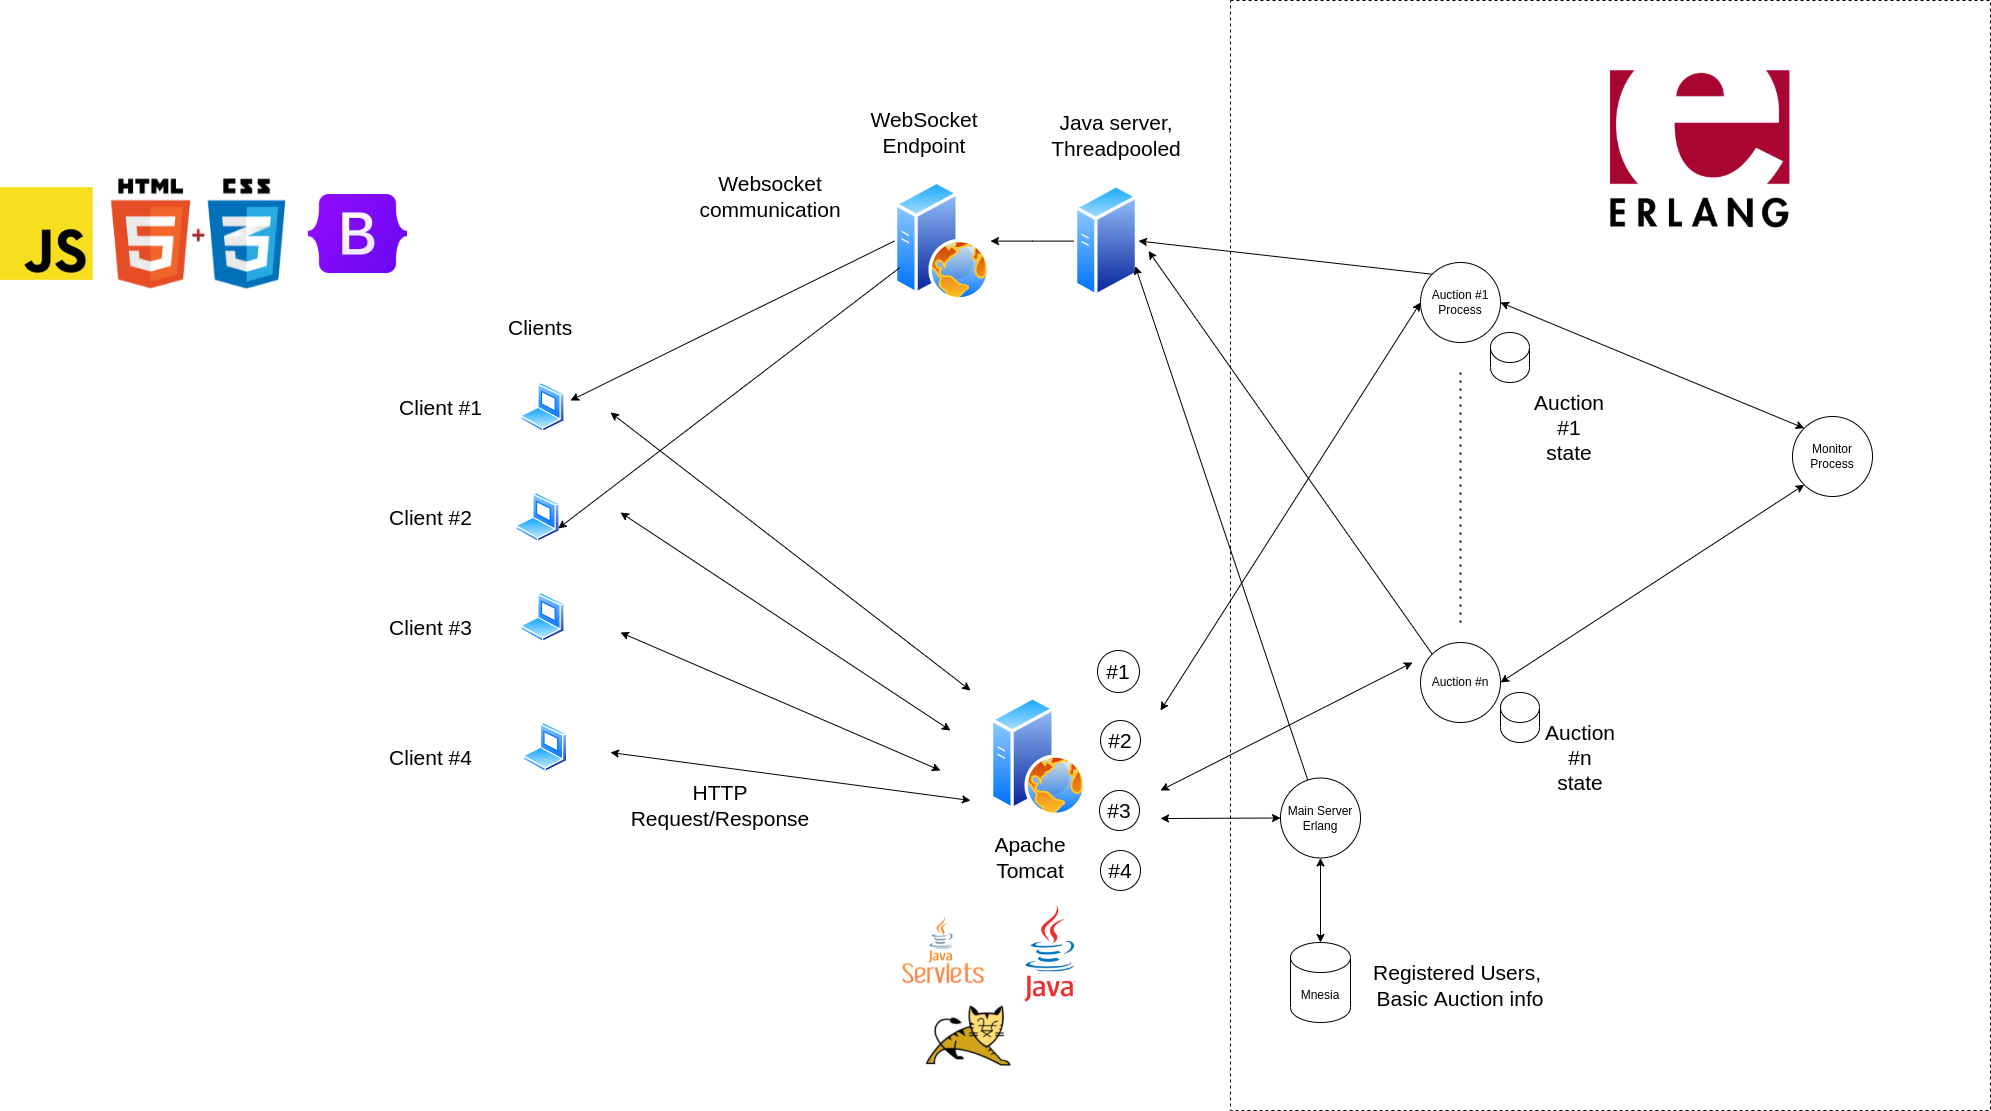
\includegraphics[width=1\linewidth]{img/systemStructure.png}
	\caption{System Architecture graphical representation}
	\label{fig:architecture}
\end{figure}

\noindent We can divide the overall system in two part:
\begin{itemize}
	\item The server side part: developed in Erlang, it is in charge of handling the request coming from the users and it has to handle the auctions and to maintain the global view of an auctions consistent among the users.
	
	\item The client side part: depeloved in Java, using EJB e JSP, and in Javascript for what regards the websocket. It is in charge of retrieving information from the server, create the GUI, update the GUI in order to let the user have a consistent view of the state of the auction and of the overall system.
\end{itemize}

\subsection{Server Side}

\subsubsection{Main Server}

\subsubsection{Auction Handler}

\subsubsection{Monitor And Supervisor}

\subsection{MnesiaDB}

\subsection{Client Side}
The web application shown to the user is generated via Apache Tomcat web-server, the page update is managed asynchronously via web-sockets, the front-end part is done with Bootstrap (a pretty famous CSS \& Javascript framework) and Javascript "vanilla". 

\subsection{Web-server with Apache Tomcat}
In Apache Tomcat web-server HTTP requests arriving from the user are processed by Java Servlets:\\

 % TODO: \usepackage{graphicx} required
 \begin{figure}[H]
 	\centering
 	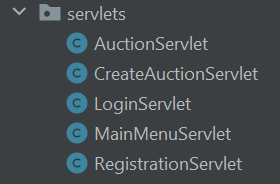
\includegraphics[width=0.4\linewidth]{img/servlets}
 	\caption{}
 	\label{fig:servlets}
 \end{figure}
 

As shown in the above figure there is one Java Servlet for each page of the web-application. From the generated page is possible to follow some hyperlinks to find other pages of the web-app.\\
The Webapp folder is organized in the following way:
% TODO: \usepackage{graphicx} required
\begin{figure}[H]
	\centering
	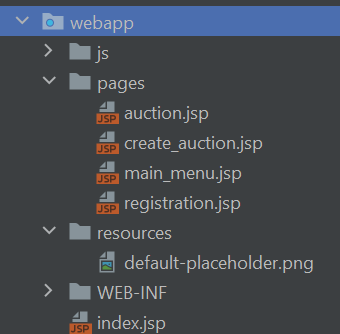
\includegraphics[width=0.4\linewidth]{img/webapp}
	\caption{}
	\label{fig:webapp}
\end{figure}

The actual HTML is generated via JSP technology, with some script-lets, for each page, in order to have a logic separation between the "View" part and the rest of the application. In example the $main\_menu.jsp$ scriptlet contains some logic to generate different cards by iterating the list of auction returned by the Erlang server.\\

In order to add some layers of security to the application a couple of Filters were added:\\
% TODO: \usepackage{graphicx} required
\begin{figure}[H]
	\centering
	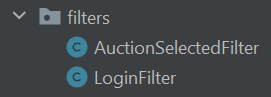
\includegraphics[width=0.4\linewidth]{img/filters}
	\caption{}
	\label{fig:filters}
\end{figure}
\begin{itemize}
	\item \textbf{LoginFilter} is responsible for checking that the request to some "protected" pages arrives with users already logged in (this can be assured by analyzing the session of the particular user, indexed by a cookie).
		
	\item \textbf{AuctionSelectedFilter} prevents a logged user to access an auction without having pressed the related button. This is done because at the same time multiple auctions can be running at the same time.\\
	
\end{itemize}
In order to update the "Model" part of our application some requests to the Server-Side part in Erlang needs to be done. This is dealt in the communication package:

% TODO: \usepackage{graphicx} required
\begin{figure}[H]
	\centering
	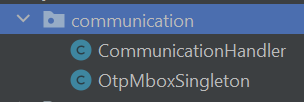
\includegraphics[width=0.4\linewidth]{img/communication}
	\caption{}
	\label{fig:communication}
\end{figure}

With the usage of Jinterface library: for each client is adopted a different mailbox of one single "Erlang" node, obtained from the cookie of the client. Then a request/reply communication happens with the Erlang Main Server and if needed with the related Auction Handler, in case an auction page is requested. The communication will return a result to communicate if the request of the client has succeeded or not (i.e. a client registration to the service may fail in case of a duplicate username).
\subsection{Web-sockets}
In order to update the application state without requesting periodically a web-page, Web-socket technology is used.

\begin{figure}[H]
	\centering
	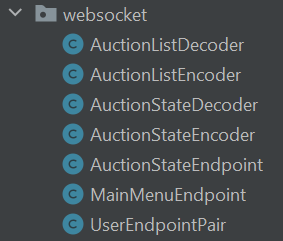
\includegraphics[width=0.4\linewidth]{img/websockets}
	\caption{}
	\label{fig:websockets}
\end{figure}

As we can see in the image above two different web-socket endpoint are used:
\begin{itemize}
	\item \textbf{MainMenuEndpoint}: responsible for updating the state of the main menu w.r.t. the list of active and inactive auctions. Clients connected to this endpoint are registered through the usage of a Java static \textit{CopyOnWriteArraySet} for dealing with concurrent changes of the connected client list.
	\item \textbf{AuctionEndpoint}: responsible for updating the state of the auction w.r.t. the list of joined users, the list of valid bids, the auction time, and the winner election. Clients connected to this endpoint are registered through the usage of a Java static ConcurrentMap<String, Set<UserEndpointPair>> data structure. With the latter, for each auction name is associated a list of client endpoints, in order to correctly send messages only to clients of a particular auction, with a publish/subscribe fashion.
\end{itemize}
\subsection{Java Listener}
There's one actor missing in the whole picture, the Java Listener.
The web-socket state update happens withe the following sequence of steps:
\begin{enumerate}
	\item A client requests a change to the state of the model (i.e. creates an auction)
	\item Apache Tomcat intercepts the requests and start the communication with the related Erlang server-side which actually stores the application state
	\item The Erlang server-side sends in general \textbf{two messages for each requests}: one is fore the servlet itself for giving an ACK to the made request, one is sent to the \textbf{java listener} for triggering the state change to other clients connected (without need of a page refresh)
	\item Java listener broadcast the state change to all interested users via web-socket
\end{enumerate}  
The advantages of using this approach are the following:
\begin{itemize}
	\item Since messages are sent by the erlang server-side (which actually is the source of truth of the web-application state), the state returned is consistent.
	\item Thanks to web-sockets, there's no need to periodically sending request to Apache Tomcat. \textbf{Page updates happens only when there is a state change}, avoiding a considerable amount computation. 
	\item Some events are triggered by erlang side itself and not by the client (i.e. auction ending and winner election), so this approach update the web-application state correctly by simply avoiding to send one message to Apache Tomcat
\end{itemize}
The \textbf{cost} of this approach is the implementation of the Java Listener.
% TODO: \usepackage{graphicx} required
\begin{figure}[H]
	\centering
	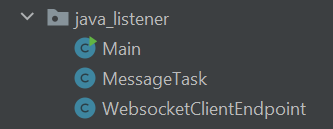
\includegraphics[width=0.4\linewidth]{img/java_listener}
	\caption{}
	\label{fig:javalistener}
\end{figure}

The Java Listener is implemented with a listener Jinterface node for getting requests from Erlang server-side. For handling multiple requests in parallel, threads are used: in particular, for avoiding the overhead due to the creation and termination of threads, \textbf{thread-pooling} is used via ExecutorService interface that implements a fixed thread pool. The task (called MessageTask) computed by each thread is related with sending a message (with the state information) to the correct web-socket endpoint.

\subsection{User Interface} 
In order to ease the UI developing a framework like \textbf{Bootstrap} has been used, in order to create a responsive web-application in a simple way, with a set of ready-to-be-used css classes, without the need of reinventing the wheel by defining our set of css classes for getting the same result. 


A couple of javascript scripts are then defined:

\begin{figure}[H]
	\centering
	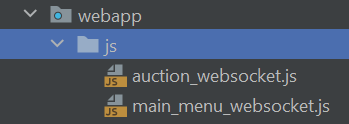
\includegraphics[width=0.4\linewidth]{img/js}
	\caption{}
	\label{fig:js}
\end{figure}

\begin{itemize}
	\item \textbf{main\_menu\_websocket}: Responsible for connecting with the main menu websocket endpoint and to update the DOM of the HTML page when a message arrives.
	\item \textbf{auction\_websocket}: Responsible for connecting the client to the auction websocket endpoint, to update the DOM of the HTML page when a message arrives and to update locally the timer.
\end{itemize}

For what concern form validation, \textbf{browser-default validation} was adopted (i.e. some fields are required to be added, some fields, like the auction duration,  must contain a number). 
\subsection{Synchronizations Issues}